% ctex_test.tex
\documentclass{article}

% Language setting
% Replace `english' with e.g. `spanish' to change the document language
\usepackage[UTF8]{ctex}
\usepackage{setspace}
\usepackage{listings}
\usepackage{xcolor}
\usepackage[colorlinks,linkcolor=blue]{hyperref}
\usepackage{enumitem}
\usepackage{tabularx}
\usepackage{longtable}
\usepackage{makecell}
\usepackage{multirow}
\usepackage{array}
\renewcommand\theadfont{\bfseries}
\renewcommand\theadgape{}

\lstset{
  backgroundcolor=\color{white},
  basicstyle=\ttfamily\footnotesize,
  breakatwhitespace=false,
  breaklines=true,
  captionpos=b,
  commentstyle=\color{mygreen},
  deletekeywords={...},
  escapeinside={\%*}{*)},
  frame=single,
  keepspaces=true,
  keywordstyle=\color{blue},
  language=Python,
  morekeywords={*,...},
  numbers=left,
  numbersep=5pt,
  numberstyle=\tiny\color{mygray},
  rulecolor=\color{black},
  showspaces=false,
  showstringspaces=false,
  showtabs=false,
  stepnumber=2,
  stringstyle=\color{mymauve},
  tabsize=2,
  title=\lstname
}


% Set page size and margins
% Replace `letterpaper' with `a4paper' for UK/EU standard size
\usepackage[letterpaper,top=2cm,bottom=2cm,left=3cm,right=3cm,marginparwidth=1.75cm]{geometry}

% Useful packages
\usepackage{amsmath}
\usepackage{graphicx}
\usepackage[colorlinks=true, allcolors=blue]{hyperref}

\title{当代人工智能实验报告3}
\author{温兆和 10205501432}

\begin{document}
\maketitle

\section{实验目的}
在本次实验中,我们使用PyTorch工具构建了多个不同的卷积神经网络架构,对MNIST手写数字数据集进行图像分类。

\section{实验环境}
出于实际需要,本次实验是在autodl上租来的云实例上进行的。

\textbf{云实例的具体配置情况:}
\begin{spacing}{0.5}
\begin{itemize}
\item 镜像:
    \begin{itemize}
        \item PyTorch 2.0.0
        \item Python 3.8(ubuntu 20.04)
        \item Cuda 11.8
    \end{itemize} 
\item GPU:RTX 4090(24GB) * 1 
\item CPU:12 vCPU Intel(R) Xeon(R) Platinum 8352V CPU @ 2.10GHz
\item 内存:90GB
\item 硬盘:
    \begin{itemize}
        \item 系统盘:30 GB
        \item 数据盘:
            \begin{itemize}
                \item 免费:50GB
                \item 付费:0GB
            \end{itemize}
    \end{itemize}
\item 附加磁盘:无
\item 端口映射:无
\item 网络:同一地区实例共享带宽
\end{itemize}
\end{spacing}

\textbf{需要安装的工具包有:}
\begin{spacing}{0.5}
\begin{itemize}
\item \lstinline|scikit_learn|
\item \lstinline|torch|
\item \lstinline|torchvision|
\end{itemize}
\end{spacing}

如果需要安装这些包,可以在项目路径下执行\lstinline|pip install -r requirements.txt|命令。
\section{实验步骤}
\subsection{数据预处理}
实际上,我们可以使用PyTorch直接下载MNIST数据集。原始的MNIST数据集分为“非测试集”和“测试集”两部分,其中前者包含$60000$条数据,后者包含$10000$条数据。我们按照$5:1$的比例把“非测试集”分为训练集和验证集,在训练模型时使用。
\begin{lstlisting}
dataset = MNIST(root="./data", train=True, transform=transform, download=True)

total_size = len(dataset)
train_size = int((5/6) * total_size) 
valid_size = total_size - train_size 
    
train_dataset, valid_dataset = random_split(dataset, [train_size, valid_size])

train_loader = DataLoader(train_dataset, batch_size=batch_size, shuffle=True)
valid_loader = DataLoader(valid_dataset, batch_size=batch_size, shuffle=False)

test_dataset = MNIST(root="./data", train=False, transform=transform, download=True)
test_loader = DataLoader(test_dataset, batch_size=batch_size, shuffle=False)
\end{lstlisting}
结果后来在训练AlexNet的时候出现了问题,训练过程中报出了输出值太小的错误:
\begin{lstlisting}
Traceback (most recent call last):
  File "D:\当代人工智能\lab 3\main.py", line 33, in <module>
    result_model = train.train(epochs, model, train_loader, optimizer, valid_loader)
  File "D:\当代人工智能\lab 3\train_and_test\train.py", line 11, in train
    outputs = model(inputs)
  File "C:\Users\HUAWEI\venv\lib\site-packages\torch\nn\modules\module.py", line 1518, in _wrapped_call_impl
    return self._call_impl(*args, **kwargs)
  File "C:\Users\HUAWEI\venv\lib\site-packages\torch\nn\modules\module.py", line 1527, in _call_impl
    return forward_call(*args, **kwargs)
  File "D:\当代人工智能\lab 3\models\AlexNet.py", line 33, in forward
    x = self.features(x)
  File "C:\Users\HUAWEI\venv\lib\site-packages\torch\nn\modules\module.py", line 1518, in _wrapped_call_impl
    return self._call_impl(*args, **kwargs)
  File "C:\Users\HUAWEI\venv\lib\site-packages\torch\nn\modules\module.py", line 1527, in _call_impl
    return forward_call(*args, **kwargs)
  File "C:\Users\HUAWEI\venv\lib\site-packages\torch\nn\modules\container.py", line 215, in forward
    input = module(input)
  File "C:\Users\HUAWEI\venv\lib\site-packages\torch\nn\modules\module.py", line 1518, in _wrapped_call_impl
    return self._call_impl(*args, **kwargs)
  File "C:\Users\HUAWEI\venv\lib\site-packages\torch\nn\modules\module.py", line 1527, in _call_impl
    return forward_call(*args, **kwargs)
  File "C:\Users\HUAWEI\venv\lib\site-packages\torch\nn\modules\pooling.py", line 166, in forward
    return F.max_pool2d(input, self.kernel_size, self.stride,
  File "C:\Users\HUAWEI\venv\lib\site-packages\torch\_jit_internal.py", line 488, in fn
    return if_false(*args, **kwargs)
  File "C:\Users\HUAWEI\venv\lib\site-packages\torch\nn\functional.py", line 791, in _max_pool2d
    return torch.max_pool2d(input, kernel_size, stride, padding, dilation, ceil_mode)
RuntimeError: Given input size: (192x2x2). Calculated output size: (192x0x0). Output size is too small
\end{lstlisting}
在进一步查阅资料后,我得知AlexNet、ResNet等模型的输入大小应该是$224*224$,而MNIST数据集中的图片长宽只有$28*28$。前向传播中,由于输入图像的尺寸过小,导致在卷积和池化层之后的特征图变得过小,经过一些卷积和池化层后,输出的特征图大小变得太小,导致池化层计算的输出大小为$0$。所以,在数据预处理时,针对不同模型,我们需要使用\lstinline|transforms.Resize()|工具对图像的尺寸进行调整。如:
\begin{lstlisting}
if args.model == 'LeNet':
    model = LeNet.LeNet()
    transform = transforms.Compose([transforms.ToTensor()])
elif args.model == 'AlexNet':
    model = AlexNet.AlexNet()
    transform = transforms.Compose([
        transforms.Resize((224, 224)),
        transforms.ToTensor(),
    ])
……
\end{lstlisting}
\subsection{模型训练与调参}
\subsubsection{LeNet}
LeNet是一种结构相对比较简单的CNN,也是本次实验中所有模型里提出时间最早的。数据经过一个卷积层、一个最大池化层、一个卷积层、一个最大池化层后,再经过三个全连接层,最终得到输出。
\begin{lstlisting}
class LeNet(nn.Module):
    def __init__(self):
        super(LeNet, self).__init__()
        self.conv1 = nn.Conv2d(1, 6, kernel_size=5)
        self.pool1 = nn.MaxPool2d(kernel_size=2, stride=2)
        self.conv2 = nn.Conv2d(6, 16, kernel_size=5)
        self.pool2 = nn.MaxPool2d(kernel_size=2, stride=2)
        self.fc1 = nn.Linear(16 * 4 * 4, 120)
        self.fc2 = nn.Linear(120, 84)
        self.fc3 = nn.Linear(84, 10)

    def forward(self, x):
        x = self.pool1(torch.relu(self.conv1(x)))
        x = self.pool2(torch.relu(self.conv2(x)))
        x = x.view(-1, 16 * 4 * 4)
        x = torch.relu(self.fc1(x))
        x = torch.relu(self.fc2(x))
        x = self.fc3(x)
        return x
\end{lstlisting}

\subsubsection{AlexNet}
相比之下,AlexNet的结构就更复杂了。它是ILSVRC-2012图像分类的冠军,也是第一个出现的大型CNN,先由五个卷积层进行特征提取,再经过三个全连接层,最终得到分类结果。
\begin{lstlisting}
class AlexNet(nn.Module):
    def __init__(self, num_classes=10):
        super(AlexNet, self).__init__()
        self.features = nn.Sequential(
            nn.Conv2d(1, 96, kernel_size=11, stride=4, padding=2),
            nn.ReLU(inplace=True),
            nn.MaxPool2d(kernel_size=3, stride=2),
            nn.Conv2d(96, 256, kernel_size=5, padding=2),
            nn.ReLU(inplace=True),
            nn.MaxPool2d(kernel_size=3, stride=2),
            nn.Conv2d(256, 384, kernel_size=3, padding=1),
            nn.ReLU(inplace=True),
            nn.Conv2d(384, 384, kernel_size=3, padding=1),
            nn.ReLU(inplace=True),
            nn.Conv2d(384, 256, kernel_size=3, padding=1),
            nn.ReLU(inplace=True),
            nn.MaxPool2d(kernel_size=3, stride=2),
        )
        self.classifier = nn.Sequential(
            nn.Dropout(),
            nn.Linear(256 * 6 * 6, 4096),
            nn.ReLU(inplace=True),
            nn.Dropout(),
            nn.Linear(4096, 4096),
            nn.ReLU(inplace=True),
            nn.Linear(4096, num_classes),
        )

    def forward(self, x):
        x = self.features(x)
        x = x.view(x.size(0), 256 * 6 * 6)
        x = self.classifier(x)
        return x
\end{lstlisting}

\subsubsection{ResNet}
ResNet是ILSVRC-2015冠军。在传统深度网络中,增加层数并不总是能够带来性能的提升,反而可能导致性能下降。随着网络深度的增加,传统的深度神经网络在训练过程中容易遇到梯度消失的问题,导致难以训练。而ResNet提出了残差学习的概念,学习网络中每个块的残差部分,而不是学习整个映射,从而让网络更容易优化。具体来说,通过引入残差块,使得增加网络深度时,网络的性能反而有所提高。

从具体实现上来看,ResNet中堆叠了许多残差块,每个残差块都有两个$3*3$卷积层,还进行了周期性的下采样。此外,残差块中还使⽤了Batch Normalization。
\begin{lstlisting}
class ResidualBlock(nn.Module):
    def __init__(self, in_channels, out_channels, stride=1):
        super(ResidualBlock, self).__init__()
        self.conv1 = nn.Conv2d(in_channels, out_channels, kernel_size=3, stride=stride, padding=1, bias=False)
        self.bn1 = nn.BatchNorm2d(out_channels)
        self.relu = nn.ReLU(inplace=True)
        self.conv2 = nn.Conv2d(out_channels, out_channels, kernel_size=3, stride=1, padding=1, bias=False)
        self.bn2 = nn.BatchNorm2d(out_channels)
        self.downsample = nn.Sequential()
        if stride != 1 or in_channels != out_channels:
            self.downsample = nn.Sequential(
                nn.Conv2d(in_channels, out_channels, kernel_size=1, stride=stride, bias=False),
                nn.BatchNorm2d(out_channels)
            )

    def forward(self, x):
        residual = x
        out = self.conv1(x)
        out = self.bn1(out)
        out = self.relu(out)
        out = self.conv2(out)
        out = self.bn2(out)
        out += self.downsample(residual)
        out = self.relu(out)
        return out


class ResNet(nn.Module):
    def __init__(self, num_classes=10):
        super(ResNet, self).__init__()
        self.in_channels = 64
        self.conv1 = nn.Conv2d(1, 64, kernel_size=7, stride=2, padding=3, bias=False)
        self.bn1 = nn.BatchNorm2d(64)
        self.relu = nn.ReLU(inplace=True)
        self.maxpool = nn.MaxPool2d(kernel_size=3, stride=2, padding=1)
        self.layer1 = self.make_layer(ResidualBlock, 64, 3, stride=1)
        self.layer2 = self.make_layer(ResidualBlock, 128, 4, stride=2)
        self.layer3 = self.make_layer(ResidualBlock, 256, 6, stride=2)
        self.layer4 = self.make_layer(ResidualBlock, 512, 3, stride=2)
        self.avgpool = nn.AdaptiveAvgPool2d((1, 1))
        self.fc = nn.Linear(512, num_classes)

    def make_layer(self, block, channels, num_blocks, stride):
        strides = [stride] + [1] * (num_blocks - 1)
        layers = []
        for stride in strides:
            layers.append(block(self.in_channels, channels, stride))
            self.in_channels = channels
        return nn.Sequential(*layers)

    def forward(self, x):
        x = self.conv1(x)
        x = self.bn1(x)
        x = self.relu(x)
        x = self.maxpool(x)
        x = self.layer1(x)
        x = self.layer2(x)
        x = self.layer3(x)
        x = self.layer4(x)
        x = self.avgpool(x)
        x = x.view(x.size(0), -1)
        x = self.fc(x)
        return x
\end{lstlisting}

\subsubsection{VGG16}
VGGNet是ILSVRC-2014图像分类亚军,它的实现思路是用更小的卷积核来加深AlexNet,VGG16是其中一个版本。具体来说,VGG16由两个两层的$3*3$卷积核和三个三层的$3*3$卷积核组成。在LeNet和AlexNet中,卷积核大小动辄达到$5$甚至是$11$。相比之下,VGG16的卷积核的确是小了很多。更小的卷积核能够在减少参数数量的同时给模型带来更多的“非线性”,这对于学习复杂的特征和模式更为有效。通过堆叠多个小卷积层,网络可以学习更复杂、更抽象的特征表示。但是,卷积核更小的代价是层数更深。深度网络通常需要更多的训练时间,因为它们需要在更多的层次上学习特征表示。
\begin{lstlisting}
class VGG16(nn.Module):
    def __init__(self, num_classes=10):
        super(VGG16, self).__init__()
        self.features = nn.Sequential(
            nn.Conv2d(1, 64, kernel_size=3, padding=1),
            nn.ReLU(inplace=True),
            nn.Conv2d(64, 64, kernel_size=3, padding=1),
            nn.ReLU(inplace=True),
            nn.MaxPool2d(kernel_size=2, stride=2),

            nn.Conv2d(64, 128, kernel_size=3, padding=1),
            nn.ReLU(inplace=True),
            nn.Conv2d(128, 128, kernel_size=3, padding=1),
            nn.ReLU(inplace=True),
            nn.MaxPool2d(kernel_size=2, stride=2),

            nn.Conv2d(128, 256, kernel_size=3, padding=1),
            nn.ReLU(inplace=True),
            nn.Conv2d(256, 256, kernel_size=3, padding=1),
            nn.ReLU(inplace=True),
            nn.Conv2d(256, 256, kernel_size=3, padding=1),
            nn.ReLU(inplace=True),
            nn.MaxPool2d(kernel_size=2, stride=2),

            nn.Conv2d(256, 512, kernel_size=3, padding=1),
            nn.ReLU(inplace=True),
            nn.Conv2d(512, 512, kernel_size=3, padding=1),
            nn.ReLU(inplace=True),
            nn.Conv2d(512, 512, kernel_size=3, padding=1),
            nn.ReLU(inplace=True),
            nn.MaxPool2d(kernel_size=2, stride=2),

            nn.Conv2d(512, 512, kernel_size=3, padding=1),
            nn.ReLU(inplace=True),
            nn.Conv2d(512, 512, kernel_size=3, padding=1),
            nn.ReLU(inplace=True),
            nn.Conv2d(512, 512, kernel_size=3, padding=1),
            nn.ReLU(inplace=True),
            nn.MaxPool2d(kernel_size=2, stride=2),
        )
        self.classifier = nn.Sequential(
            nn.Linear(512 * 7 * 7, 4096),
            nn.ReLU(inplace=True),
            nn.Dropout(),
            nn.Linear(4096, 4096),
            nn.ReLU(inplace=True),
            nn.Dropout(),
            nn.Linear(4096, num_classes),
        )

    def forward(self, x):
        x = self.features(x)
        x = x.view(x.size(0), -1)
        x = self.classifier(x)
        return x
\end{lstlisting}

\subsubsection{GoogleNet}
GoogleNet在VGGNet的基础上又进行了改进。它利用“高维数据一般非常稀疏”的特点,聚合多个⼩型稠密连接,把全连接层层替换成更加稀疏的连接层,从而降低了网络的深度。具体来说,它包括两个卷积层\lstinline|conv1|和\lstinline|conv2|,分别用于提取不同尺度的特征。然后,通过堆叠两个\lstinline|InceptionModule|来提取更高层次的特征。最后,经过全局平均池化和全连接层输出分类结果。
\begin{lstlisting}
import torch.nn.functional as F


class InceptionModule(nn.Module):
    def __init__(self, channels_in):
        super().__init__()
        self.branch1 = nn.Sequential(
            nn.AvgPool2d(3, stride=1, padding=1),
            nn.Conv2d(channels_in, 24, 1)
        )
        self.branch2 = nn.Conv2d(channels_in, 16, 1)
        self.branch3 = nn.Sequential(
            nn.Conv2d(channels_in, 16, 1),
            nn.Conv2d(16, 24, 5, padding=2)
        )
        self.branch4 = nn.Sequential(
            nn.Conv2d(channels_in, 16, 1),
            nn.Conv2d(16, 23, 3, padding=1),
            nn.Conv2d(23, 24, 3, padding=1)
        )

    def forward(self, x):
        return torch.cat([self.branch1(x), self.branch2(x), self.branch3(x), self.branch4(x)], 1)


class GoogleNet(nn.Module):
    def __init__(self):
        super().__init__()
        self.conv1 = nn.Conv2d(1, 10, 5)
        self.conv2 = nn.Conv2d(88, 20, 5)
        self.incep1 = InceptionModule(channels_in=10)
        self.incep2 = InceptionModule(channels_in=20)
        self.maxpool = nn.MaxPool2d(2)
        self.fully_connection = nn.Linear(1408, 10)

    def forward(self, x):
        size_fc = x.shape[0]
        x = F.relu(self.maxpool(self.conv1(x)))
        x = self.incep1(x)
        x = F.relu(self.maxpool(self.conv2(x)))
        x = self.incep2(x)
        x = x.view(size_fc, -1)
        x = self.fully_connection(x)
        return x
\end{lstlisting}

\subsection{模型测试}
通过选择合适的参数,我们对各个模型的性能进行了测试。需要说明的是,由于VGG16的运行时间过长,两个小时都没有打印出第一个epoch的验证准确率,我们不再设法获取和研究VGG16的准确率。其余每个模型各训练十个epoch,每个epoch结束后在验证集上验证一次,训练后输出模型在测试集上的预测结果。

\subsubsection{各个模型的运行结果}
\begin{longtable}{|c|c|c|c|c|c|}
  \caption{各个模型的运行结果}\label{tab:mytable} \\
  \hline
  \textbf{模型} & \multicolumn{4}{c|}{\textbf{参数配置}} & \textbf{运行结果} \\
  \cline{2-5}
  ~ & \makecell{learning\\ rate} & \makecell{batch\\ size} & \makecell{optimizer} & \makecell{gamma} & ~ \\
  \hline
  \endfirsthead
  
  \multicolumn{6}{c}%
  {{\tablename\ \thetable{} -- 续页}} \\
  \hline
  \textbf{模型} & \multicolumn{4}{c|}{\textbf{参数配置}} & \textbf{运行结果} \\
  \cline{2-5}
  ~ & \makecell{learning\\ rate} & \makecell{batch\\ size} & \makecell{optimizer} & \makecell{gamma} & ~ \\
  \hline
  \endhead
  
  LeNet & 0.05 & 64 & SGD & 1.0 & \raisebox{-\height}{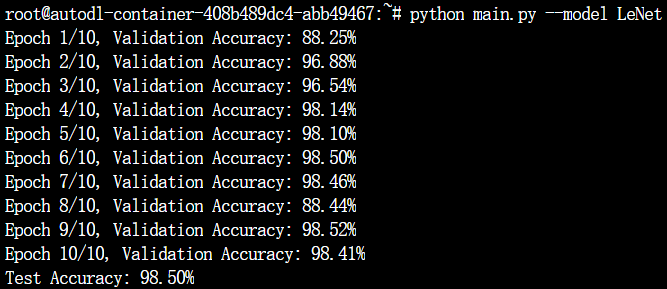
\includegraphics[width=0.5\textwidth,valign=c]{LeResult.png}} \\
  \hline
  AlexNet & 0.05 & 64 & SGD & 1.0 & \raisebox{-\height}{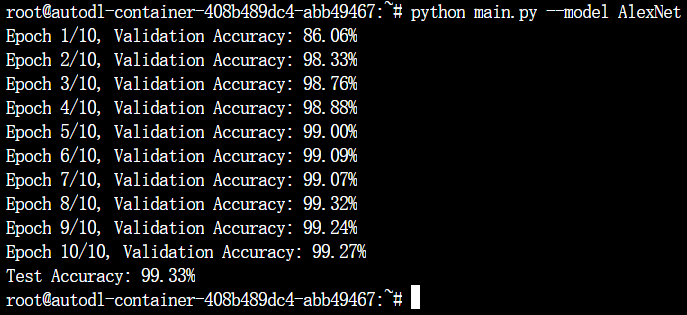
\includegraphics[width=0.5\textwidth,valign=c]{AlexResult.png}} \\
  \hline
  ResNet & 0.05 & 64 & SGD & 1.0 & \raisebox{-\height}{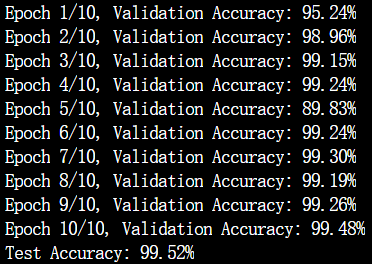
\includegraphics[width=0.5\textwidth,valign=c]{ResResult.png}} \\
  \hline
  GoogleNet & 0.005 & 64 & Adam & 1.0 & \raisebox{-\height}{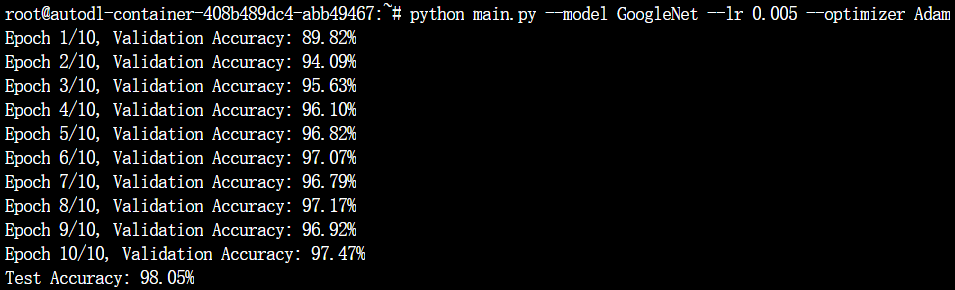
\includegraphics[width=0.5\textwidth,valign=c]{GoogleResult.png}} \\
  \hline
\end{longtable}
将模型的运行结果用图表进行可视化,如下:
\begin{figure}[h]
    \lefting
    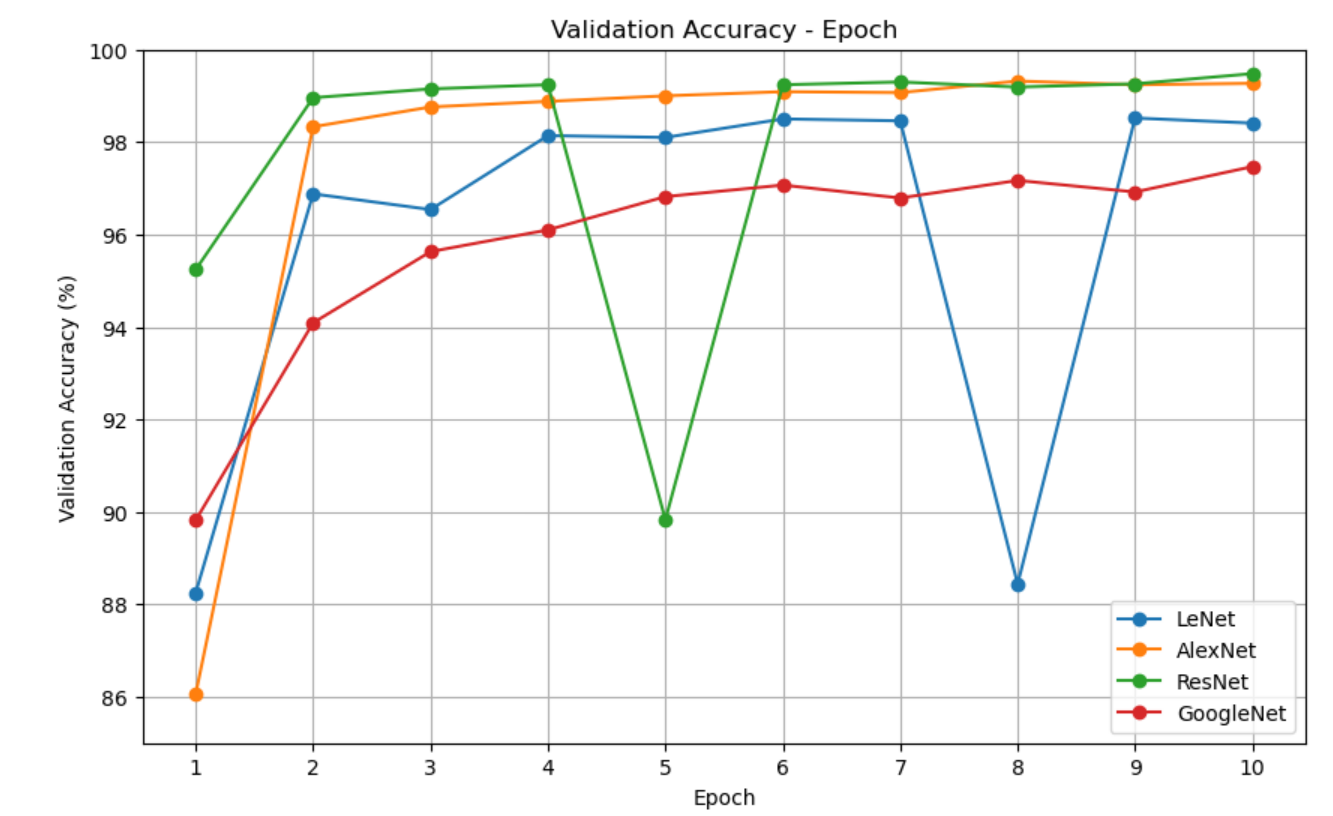
\includegraphics[width=0.5\linewidth]{ValAcc.png}
    % \caption{训练过程中验证准确率的变化}
    \label{fig:enter-label}
% \end{figure}
% \begin{figure}
    \righting
    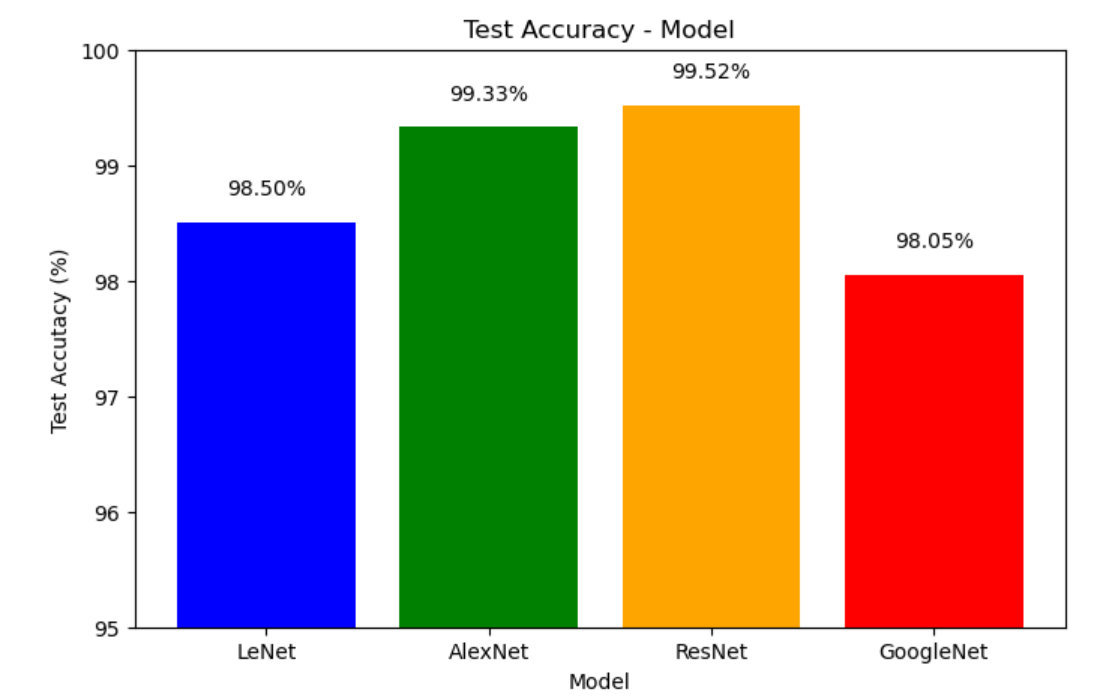
\includegraphics[width=0.5\linewidth]{TestRes.png}
    \caption{左:训练过程中验证准确率的变化,右:各模型测试准确率}
    \label{fig:enter-label}
\end{figure}
\subsubsection{结果分析}
从上面的结果可以看出,模型的预测准确率和它的结构复杂度是呈正相关的。由于担心GoogleNet会像VGG16一样好久都跑不出结果,我们特意简化了GoogleNet的结构,所以它的准确率最低。LeNet也是一种结构比较简单的神经网络,所以它的复杂度也不算高。AlexNet比LeNet多了几个卷积层,能够更好地提取图像的特征,所以它的准确率比LeNet高出不少,能够达到$99\%$以上。ResNet是本次实验中结构最复杂的卷积神经网络,所以它有最高的准确率。但是,ResNet的训练时间比AlexNet长了不少,但准确率没有比AlexNet高很多。如果把训练模型的时间开销也考虑在内,那么AlexNet应该是一种总体性能相当好的卷积神经网络。当然,如果我们不去简化GoogleNet的结构,也许它也能达到一个比较高的准确率。

\section{总结}
在本次实验中,我们使用深度学习开源软件搭建了五个可用于图像分类的卷积神经网络并测试了它们的性能,体会到神经网络在面对复杂非线性数据集时的强大。

\end{document}